\section{Rastreamento dos Usuários}

	O Sistema TRUE detecta os usuários no ambiente utilizando o metodo de subtração
	de fundo, descrito na Secão~\ref{sec:deteccao-objeto}, os rastreia e os
	respresenta por suas silhuetas, descrita na	Seção~\ref{sec:representacao-objeto}.
	Existem dois pontos principais em que se deve averiguar a confiabilidade do
	rastreamento. A primeira é sobre a detecção de usuários, sua velocidade e
	confiabilidade, e a segunda é sobre a interferência entre os usuários na cena.
	
	\subsection{Testes da Detecção}
	
		Todo e qualquer movimento que ocorra na cena será detectado. Usuários que
		iniciarem e permanecerem imovéis não serão detectados.
		
		\begin{figure}[H]
			\begin{center}
				\subfloat[] {
					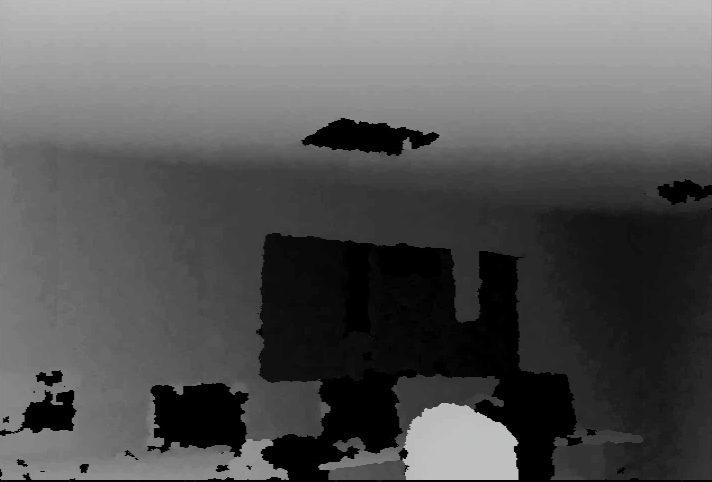
\includegraphics[width=0.25\textwidth]{figuras/5.Testes/deteccao/1.png}}
				\subfloat[] {
					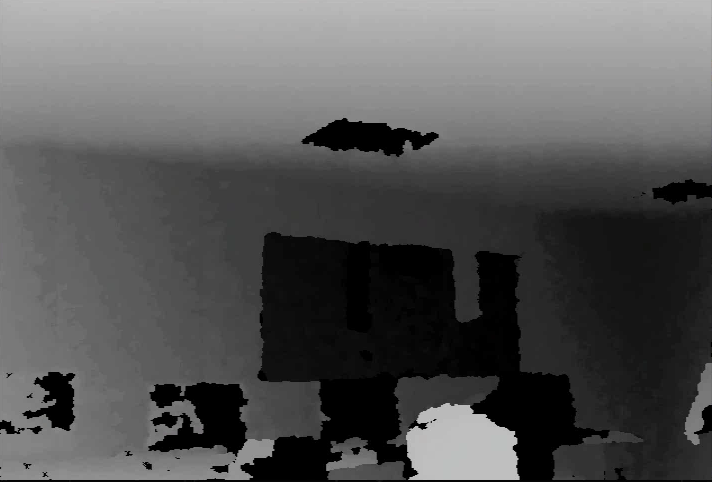
\includegraphics[width=0.25\textwidth]{figuras/5.Testes/deteccao/2.png}}
				\subfloat[] {
					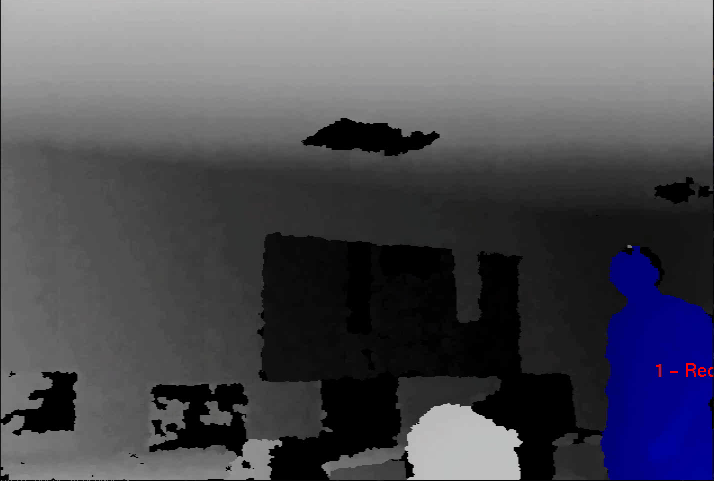
\includegraphics[width=0.25\textwidth]{figuras/5.Testes/deteccao/3.png}}
				\subfloat[] {
					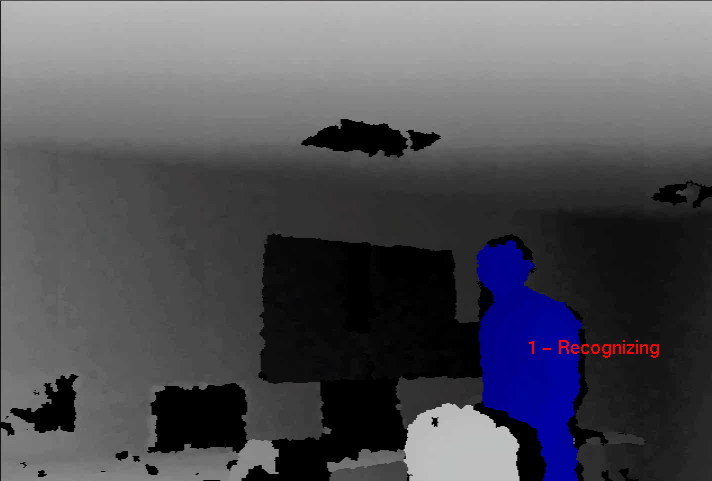
\includegraphics[width=0.25\textwidth]{figuras/5.Testes/deteccao/4.png}}
			\end{center}
			\caption{Detecção de novos usuários.}
			\label{fig:testes_deteccao}
		\end{figure}
		
	\subsection{Testes do Máximo de Usuários}
	
	\subsection{Teste de Oclusão}
	
		\begin{figure}[H]
		\begin{center}
				\subfloat[] {
					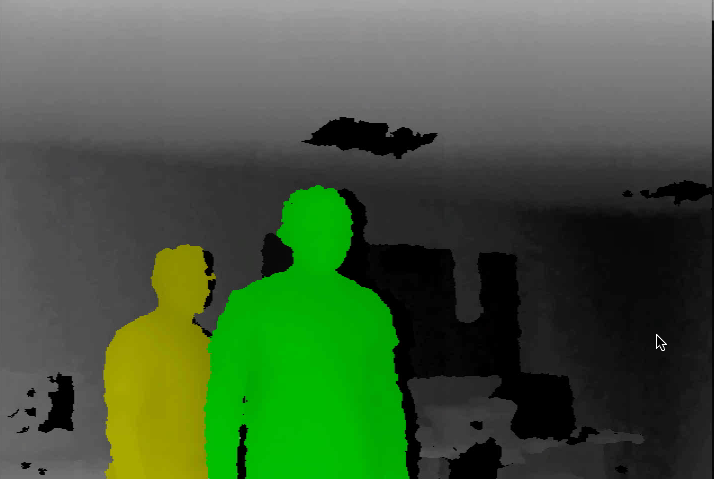
\includegraphics[width=0.19\textwidth]{figuras/5.Testes/oclusao/1.png}}
				\subfloat[] {
					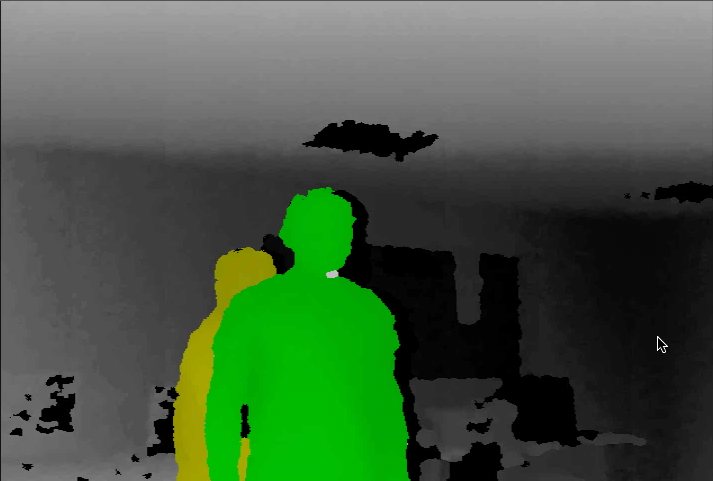
\includegraphics[width=0.19\textwidth]{figuras/5.Testes/oclusao/2.png}}
				\subfloat[] {
					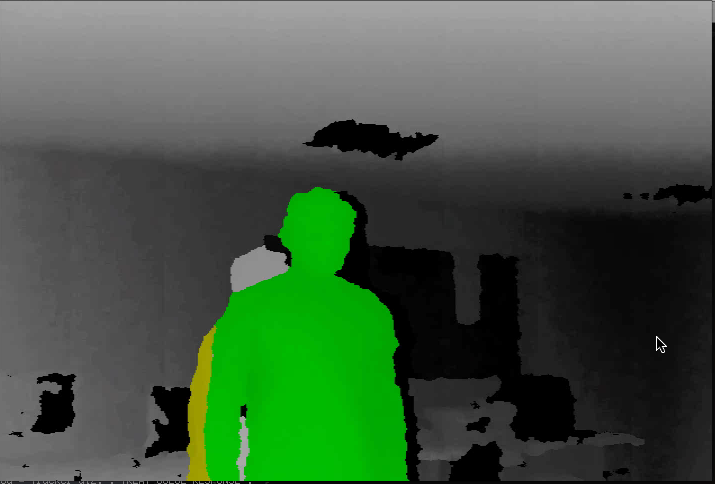
\includegraphics[width=0.19\textwidth]{figuras/5.Testes/oclusao/3.png}}
				\subfloat[] {
					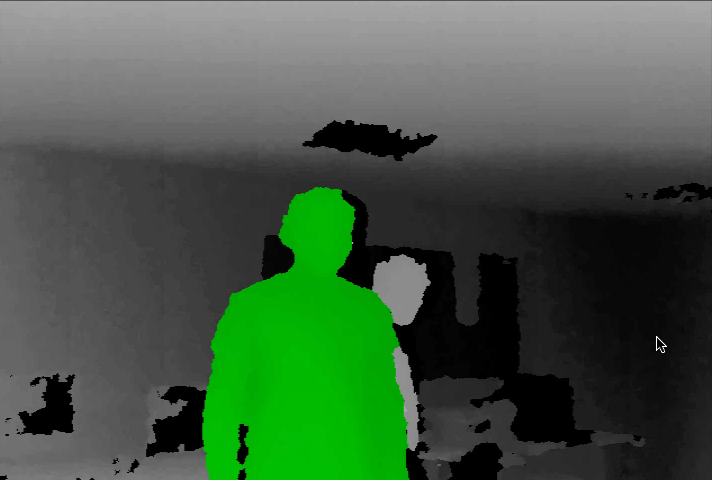
\includegraphics[width=0.19\textwidth]{figuras/5.Testes/oclusao/4.png}}
				\subfloat[] {
					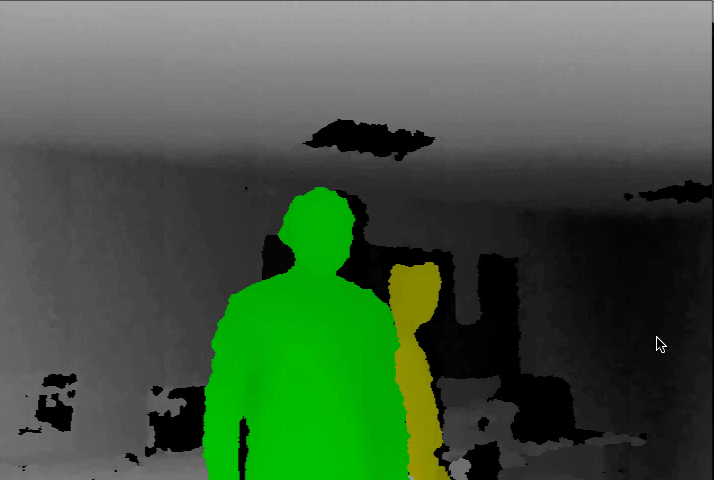
\includegraphics[width=0.19\textwidth]{figuras/5.Testes/oclusao/5.png}}
			\end{center}
			\caption{Oclusão de usuários.}
			\label{fig:testes_oclusao}
		\end{figure}
		
		
		\begin{figure}[H]
			\begin{center}
				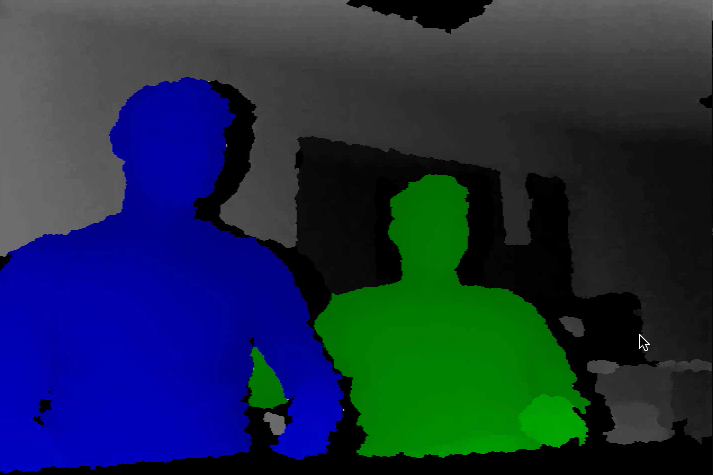
\includegraphics[width=0.75\textwidth]{figuras/5.Testes/oclusao/oclusao_corretamente.png}
			\end{center}
			\caption{Oclusão de usuários ocorrendo com sucesso.}
			\label{fig:testes_oclusao_sucesso}
		\end{figure}
		
	
	\subsection{Testes de Relacionamento com Objetos}
	
		\begin{figure}[H]
			\begin{center}
				\subfloat[] {
					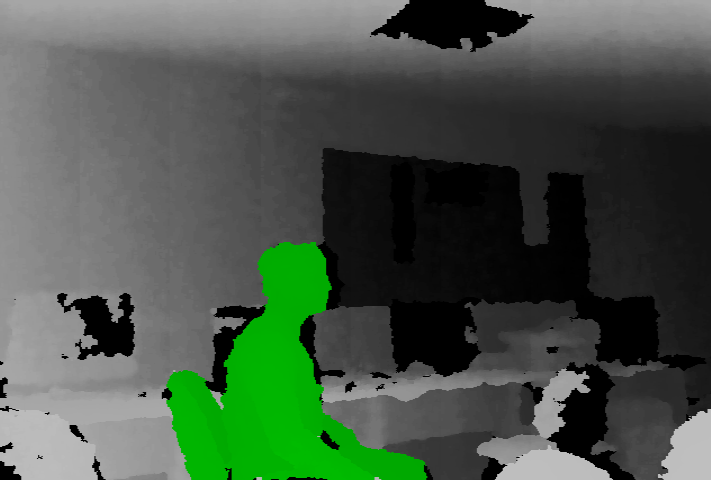
\includegraphics[width=0.37\textwidth]{figuras/5.Testes/relacionamento_com_objetos/1.png}}
				\subfloat[] {
					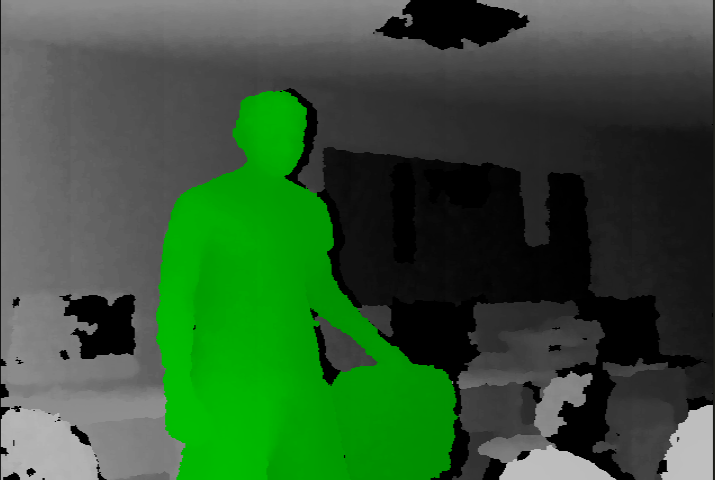
\includegraphics[width=0.37\textwidth]{figuras/5.Testes/relacionamento_com_objetos/2.png}}
			\end{center}
			\caption{Usuários sendo rastreado conjuntamente com os objetos que interege.}
			\label{fig:testes_relacionamento_com_objetos}
		\end{figure}
		
	
	\subsection{Testes de Interferência}
	
		Os métodos utilizados permitem uma certa interferência entre os usuários
		quando os mesmos estão muito perto ou quando se tocam.

		\begin{figure}[H]
			\begin{center}
				\subfloat[] {
					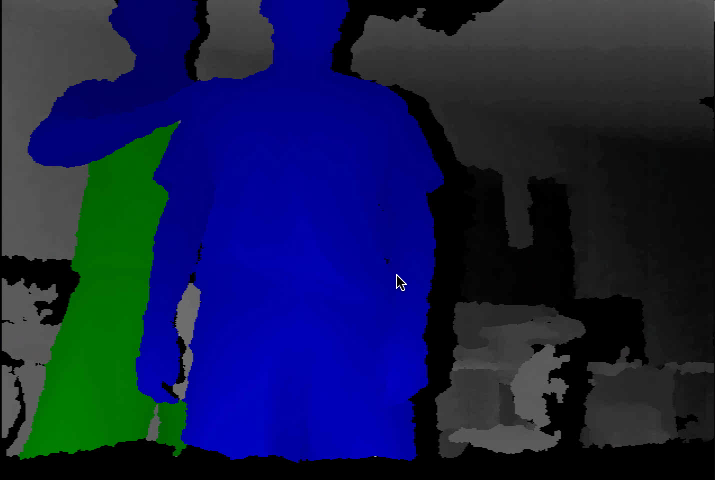
\includegraphics[width=0.32\textwidth]{figuras/5.Testes/relacionamento_com_pessoas/1.png}}
				\subfloat[] {
					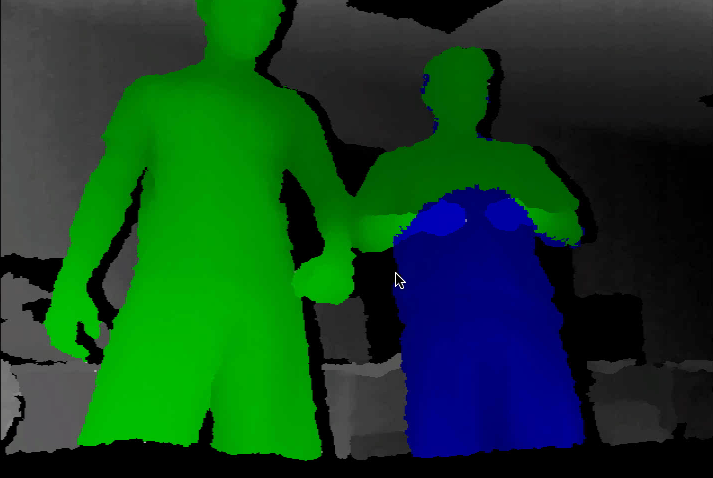
\includegraphics[width=0.32\textwidth]{figuras/5.Testes/relacionamento_com_pessoas/2.png}}
				\subfloat[] {
					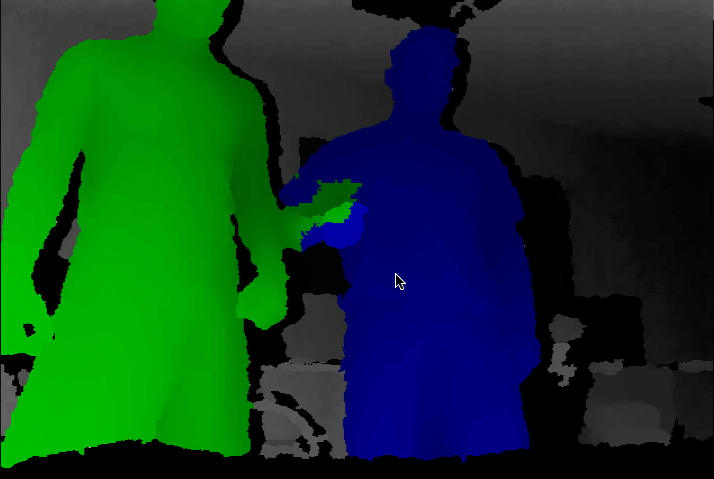
\includegraphics[width=0.32\textwidth]{figuras/5.Testes/relacionamento_com_pessoas/3.png}}
			\end{center}
			\caption{Usuários sofrendo interferência dos que estão ao seu redor.}
			\label{fig:testes_relacionamento_com_usuarios}
		\end{figure}